---
id: tkz-euclide-ejemplo-28
title: "Circuncentro"
description: "Calcula el baricentro y traza las tres medianas de un triángulo, marcando puntos medios y congruencias."
keywords: [baricentro, medianas, triángulo, puntos-medios, isosceles]
tags: [tkzDefTriangle, tkzDefTriangleCenter,tkzDefMidPoint,tkzDrawPolygon,tkzGetPoint,median]
sort: 28
---
\documentclass[tikz,border=2mm]{standalone}
\usepackage{tkz-euclide}

\begin{document}
    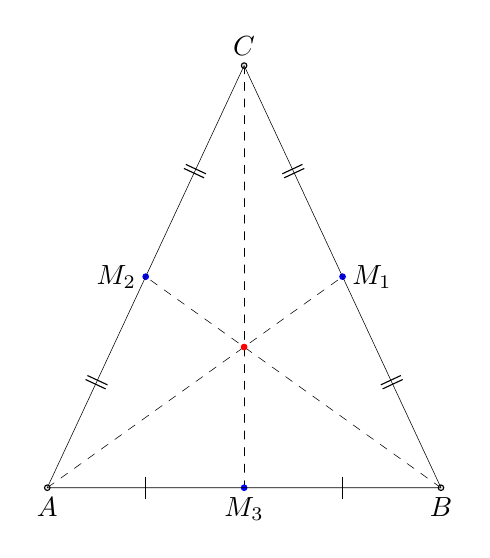
\begin{tikzpicture}
        % Define la base AB del triángulo.
        \tkzDefPoint(0,0){A}
        \tkzDefPoint(5,0){B}
    
        % Construye un triángulo con ángulos en A y B de 65°.
        \tkzDefTriangle[two angles = 65 and 65](A,B)
            \tkzGetPoint{C}
    
        % Encuentra el baricentro (centro de las medianas) O.
        \tkzDefTriangleCenter[median](A,B,C)
            \tkzGetPoint{O}
    
        % Calcula los puntos medios de los lados y obtén a, b y c.
        \tkzDefMidPoint(B,C)
            \tkzGetPoint{a}
        \tkzDefMidPoint(A,C)
            \tkzGetPoint{b}
        \tkzDefMidPoint(A,B)
            \tkzGetPoint{c}
    
        % Dibuja las medianas como segmentos punteados.
        \tkzDrawSegment[dashed](A,a)
        \tkzDrawSegment[dashed](B,b)
        \tkzDrawSegment[dashed](C,c)
    
        % Dibuja y etiqueta puntos medios.
        \tkzDrawPoints[blue](a,b,c)
        \tkzLabelPoint[right](a){$M_1$}
        \tkzLabelPoint[left](b){$M_2$}
        \tkzLabelPoint[below](c){$M_3$}
    
        % Marca la igualdad de segmentos en cada lado.
        \tkzMarkSegments[mark=||](C,a a,B)
        \tkzMarkSegments[mark=||](C,b b,A)
        \tkzMarkSegments[mark=|](A,c c,B)
    
        % Dibuja el baricentro, el triángulo y etiqueta vértices.
        \tkzDrawPoints[red](O)
        \tkzDrawPoints(A,B,C)
        \tkzDrawPolygon(A,B,C)
        \tkzLabelPoints(A,B)
        \tkzLabelPoints[above](C)
    \end{tikzpicture}
\end{document}
